AGREE translates an AADL model and its annotated contracts into a dialect \cite{jkind} of the Lustre language, and then queries a user-selected model checker to perform the verification. The dialect introduced an expression called \emph{condact}, which is similar to the activation condition in SCADE. It clocks a node call expression as follows: 
\begin{equation*}
condact (cond, node(node\_inputs, node\_outputs), init\_outputs)
\end{equation*}
If the Boolean signal $cond$ is true, the clocked node $node$ is activated and updates its local and output signals. Otherwise, the node keeps the previous value of the local and output signals. Before the first activation, the node outputs values are set to \emph{init\_outputs}. %\emph{condact} is essential to model the scheduling semantics. 
We are aware that the standard Lustre language introduced similar temporal operators like \emph{when} and \emph{current}. We use \emph{condact} simply because it is supported by our default model checker JKind \cite{jkind}.

AGREE translates an AADL thread to a Lustre node in a \emph{constraint} style, where the thread input and output ports are both mapped to the node input signals. Thus, the \emph{condact} expression does not automatically freeze the thread outputs. We add assertions to enforce the output freeze rule. And we use the thread \emph{complete} signal to clock the node. The \emph{complete} signal is triggered by the circular counter shown in Figure \ref{schedule} . Figure \ref{WPMlustre} shows an example of using \emph{condact} to model a scheduled AADL thread. 

\begin{figure}[ht!]
\centering
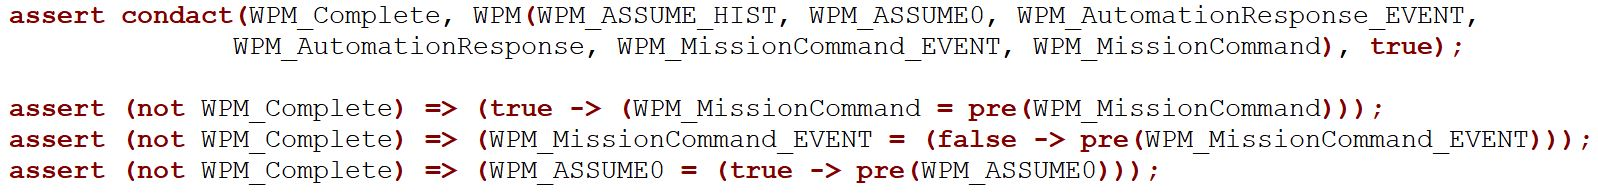
\includegraphics[width=120mm]{lustreAsync5.jpg}
\caption{A Lustre Model of a Scheduled AADL Thread \label{WPMlustre}}
\end{figure}

%\begin{figure}[ht!]
%\centering
%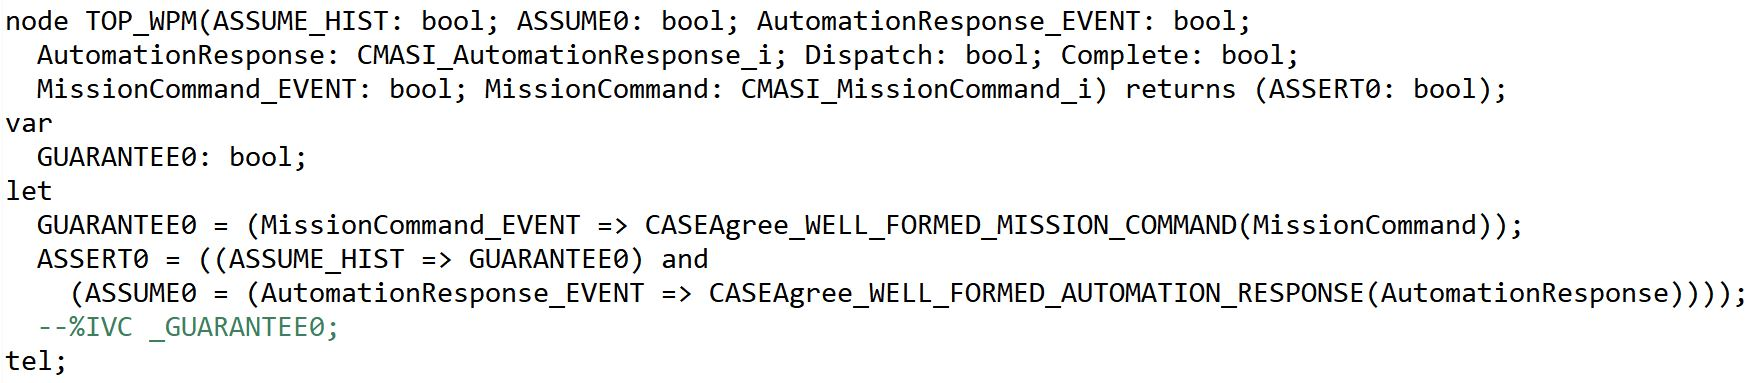
\includegraphics[width=130mm]{wpmLustre2.jpg}
%\caption{A Lustre Model of AADL Thread \label{WPMlustre}}
%\end{figure}
%
%\begin{figure}[ht!]
%\centering
%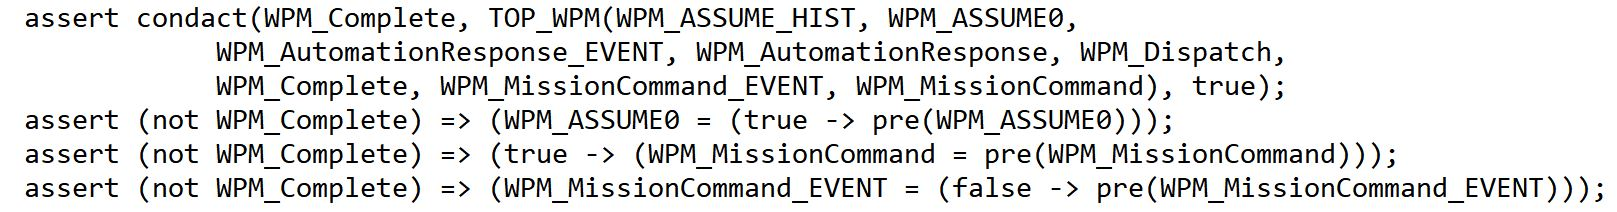
\includegraphics[width=130mm]{lustreAsync4.jpg}
%\caption{A Lustre Expression \emph{condact} Usage Example\label{lustreAsync}}
%\end{figure}
%
%\begin{figure}[ht!]
%\centering
%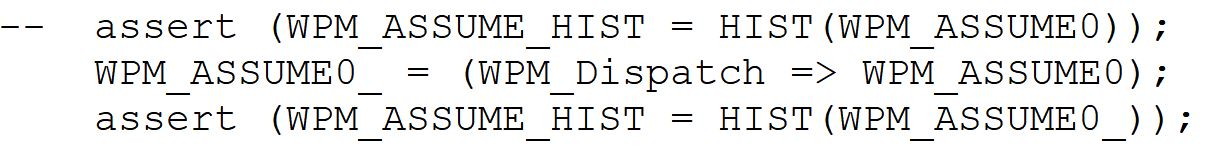
\includegraphics[width=80mm]{LustreAssume.jpg}
%\caption{An Example of Assumption Model in Lustre \label{lustreAsync}}
%\end{figure}

%\begin{figure}[ht!]
%\centering
%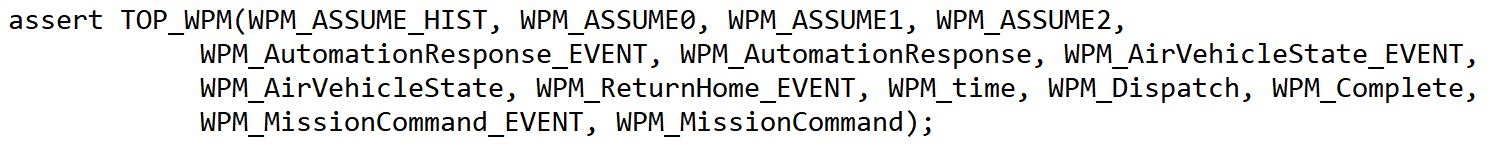
\includegraphics[width=120mm]{lustreSync2.jpg}
%\caption{An AADL Model Illustrating Motivation\label{lustreSync}}
%\end{figure}

%\begin{lstlisting}[language=c,frame=single,caption=An AGREE model of a schedule,label=schedule_model]
%  assert condact(WPM__Complete, _TOP__WPM(WPM____ASSUME__HIST, WPM____ASSUME0, WPM____ASSUME1, WPM____ASSUME2, 
%				WPM__AutomationResponse___EVENT_, WPM__AutomationResponse, WPM__AirVehicleState___EVENT_, WPM__AirVehicleState, 
%                WPM__ReturnHome___EVENT_, WPM__time, WPM__Dispatch, WPM__Complete, WPM__MissionCommand___EVENT_, WPM__MissionCommand), true);
%  assert (not WPM__Complete) => (WPM____ASSUME0 = (true -> pre(WPM____ASSUME0)));
%  assert (not WPM__Complete) => (WPM____ASSUME1 = (true -> pre(WPM____ASSUME1)));
%  assert (not WPM__Complete) => (WPM____ASSUME2 = (true -> pre(WPM____ASSUME2)));
%  assert (not WPM__Complete) => (true -> (WPM__MissionCommand = pre(WPM__MissionCommand)));
%  assert (not WPM__Complete) => (WPM__MissionCommand___EVENT_ = (false -> pre(WPM__MissionCommand___EVENT_)));
%\end{lstlisting}  
  